\subsection{Функции потерь}\label{subsec:losses}

\begin{definition}
  Функция потерь $f_{loss}(y, \hat{y})$ --- функция, характеризующая величину отклонения ответа $y$ нейронной сети от правильного ответа~$\hat{y}$.
\end{definition}

Целью обучения нейронной обучения является минимизация функции потерь. Основным методом такой минимизации является градиентный спуск\cite[с.\,151]{bib:neural_networks2}.

Под цели задачи подходят следующие функции в качестве функции потерь:
\begin{eqnarray}
% \nonumber % Remove numbering (before each equation)
  \nonumber f_{log}(y, \hat{y}) &=& -\log(1 - |y-\hat{y}|), \\
  \nonumber f_{exp}(y, \hat{y}) &=& e^{|y-\hat{y}|} - 1.
\end{eqnarray}

Ниже представлены графики этих функций и их реализации\cite[раздел backend]{bib:keras} на языке Python.
\begin{figure}[h]
\begin{tikzpicture}
\begin{axis}[
    axis lines = left,
    xlabel = $x$,
    ylabel = {$f(x)$},
    width = 14cm,
    height = 11cm,
    xmin = 0,
    ymax = 5,
    legend pos=south east
]
%Below the red parabola is defined
\addplot [
    domain=-0.2:2.1,
    samples=100,
    color=red
]
{-ln(1-x)};
\addlegendentry{$f_{log}$}
%Here the blue parabloa is defined
\addplot [
    domain=-0.2:2.1,
    samples=100,
    color=blue
    ]
    {e^x -1};
\addlegendentry{$f_{exp}$}
\addplot [dashed] coordinates {(1, 0) (1, 6)};

\end{axis}
\end{tikzpicture}
\caption{Графики функций потерь}\label{fig:custom_losses}
\end{figure}

\begin{figure}[h]
    \centering
    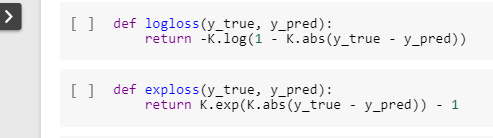
\includegraphics[width=0.9\textwidth]{losses_python.png}
    \caption{Реализации функций потерь}\label{fig:custom_losses}
    \label{fig:losses_python}
\end{figure}

%\lstinputlisting[language=Python]{logloss_exploss.py}
